%%%%%%%%%%%%%%%%%%%%%%% file template.tex %%%%%%%%%%%%%%%%%%%%%%%%%
%
% This is a template file for the LaTeX package SVJour2 for the
% Springer journal "The VLDB Journal".
%
%                                    Springer Heidelberg 2004/12/03
%
% Copy it to a new file with a new name and use it as the basis
% for your article. Delete % as needed.
%
%%%%%%%%%%%%%%%%%%%%%%%%%%%%%%%%%%%%%%%%%%%%%%%%%%%%%%%%%%%%%%%%%%%
%
% First comes an example EPS file -- just ignore it and
% proceed on the \documentclass line
% your LaTeX will extract the file if required
%\begin{filecontents*}{figs/minimalperfecthash-ph-mph.ps}
%!PS-Adobe-3.0 EPSF-3.0
%%BoundingBox: 19 19 221 221
%%CreationDate: Mon Sep 29 1997
%%Creator: programmed by hand (JK)
%%EndComments
%gsave
%newpath
%  20 20 moveto
%  20 220 lineto
%  220 220 lineto
%  220 20 lineto
%closepath
%2 setlinewidth
%gsave
%  .4 setgray fill
%grestore
%stroke
%grestore
%\end{filecontents*}
%
\documentclass[twocolumn,fleqn,runningheads]{svjour2}
%
\smartqed  % flush right qed marks, e.g. at end of proof
%
\usepackage{graphicx}
\usepackage{listings}
\usepackage{epsfig}
\usepackage{textcomp}
\usepackage[latin1]{inputenc}
\usepackage{amssymb}

\DeclareGraphicsExtensions{.png} 
%
% \usepackage{mathptmx}      % use Times fonts if available on your TeX system
%
% insert here the call for the packages your document requires
%\usepackage{latexsym}
% etc.
%
% please place your own definitions here and don't use \def but
% \newcommand{}{}
%

\lstset{
  language=Pascal,
  basicstyle=\fontsize{9}{9}\selectfont,
  captionpos=t,
  aboveskip=1mm,
  belowskip=1mm,
  abovecaptionskip=1mm,
  belowcaptionskip=1mm,
%  numbers = left,
  mathescape=true,
  escapechar=@,
  extendedchars=true,
  showstringspaces=false,
  columns=fixed,
  basewidth=0.515em,
  frame=single,
  framesep=2mm,
  xleftmargin=2mm,
  xrightmargin=2mm,
  framerule=0.5pt
}

\def\cG{{\mathcal G}}
\def\crit{{\rm crit}}
\def\ncrit{{\rm ncrit}}
\def\scrit{{\rm scrit}}
\def\bedges{{\rm bedges}}
\def\ZZ{{\mathbb Z}}

\journalname{The VLDB Journal}
%

\begin{document}

\title{Space and Time Efficient Minimal Perfect Hash \\[0.2cm]
Functions for Very Large Databases\thanks{
This work was supported in part by
GERINDO Project--grant MCT/CNPq/CT-INFO 552.087/02-5,
CAPES/PROF Scholarship (Fabiano C. Botelho),
FAPESP Proj.\ Tem.\ 03/09925-5 and CNPq Grant 30.0334/93-1
(Yoshiharu Kohayakawa),
and CNPq Grant 30.5237/02-0 (Nivio Ziviani).}
}
%\subtitle{Do you have a subtitle?\\ If so, write it here}

%\titlerunning{Short form of title}        % if too long for running head

\author{Fabiano C. Botelho \and Davi C. Reis \and Yoshiharu Kohayakawa \and Nivio Ziviani}
%\authorrunning{Short form of author list} % if too long for running head
\institute{
F. C. Botelho \and 
N. Ziviani \at
Dept. of Computer Science,
Federal Univ. of Minas Gerais,
Belo Horizonte, Brazil\\
\email{\{fbotelho,nivio\}@dcc.ufmg.br}
\and
D. C. Reis \at
Google, Brazil \\
\email{davi.reis@gmail.com}
\and
Y. Kohayakawa
Dept. of Computer Science,
Univ. of S\~ao Paulo,
S\~ao Paulo, Brazil\\
\email{yoshi@ime.usp.br}
}

\date{Received: date / Accepted: date}
% The correct dates will be entered by the editor


\maketitle

\begin{abstract}
We propose a novel external memory based algorithm for constructing minimal
perfect hash functions~$h$ for huge sets of keys.
For a set of~$n$ keys, our algorithm outputs~$h$ in time~$O(n)$.
The algorithm needs a small vector of one byte entries
in main memory to construct $h$.
The evaluation of~$h(x)$ requires three memory accesses for any key~$x$.
The description of~$h$ takes a constant number of bits
for each key, which is optimal, i.e., the theoretical lower bound is $1/\ln 2$
bits per key.
In our experiments, we used a collection of 1 billion URLs collected
from the web, each URL 64 characters long on average.
For this collection, our algorithm
(i) finds a minimal perfect hash function in approximately
3 hours using a commodity PC,
(ii) needs just 5.45 megabytes of internal memory to generate $h$
and (iii) takes 8.1 bits per key for the description of~$h$.
\keywords{Minimal Perfect Hashing \and Large Databases}
\end{abstract}

% main text

\def\cG{{\mathcal G}}
\def\crit{{\rm crit}}
\def\ncrit{{\rm ncrit}}
\def\scrit{{\rm scrit}}
\def\bedges{{\rm bedges}}
\def\ZZ{{\mathbb Z}}
\def\BSmax{\mathit{BS}_{\mathit{max}}}
\def\Bi{\mathop{\rm Bi}\nolimits}

\section{Introduction} \label{sec:introduction}


The important performance parameters of a PHF are representation size, evaluation time and construction time. The representation size plays an important role when the whole function fits in a faster memory and the actual data is stored in a slower memory. For instace, compact PHFs can be entirely fit in a CPU cache and this makes their computation really fast by avoiding cache misses. The CHD algorithm plays an important role in this context. It was designed by Djamal Belazzougui, Fabiano C. Botelho, and Martin Dietzfelbinger in \cite{bbd09}.


The CHD algorithm permits to obtain PHFs with representation size very close to optimal while retaining $O(n)$ construction time and $O(1)$ evaluation time. For example, in the case $m=2n$ we obtain a PHF that uses space $0.67$ bits per key, and for $m=1.23n$ we obtain space $1.4$ bits per key, which was not achievable with previously known methods. The CHD algorithm is inspired by several known algorithms; 
the main new feature is that it combines a modification of Pagh's ``hash-and-displace'' approach
with data compression on a sequence of hash function indices. 
That combination makes it possible to significantly reduce space usage 
while retaining linear construction time and constant query time. 
The CHD algorithm can also be used for $k$-perfect hashing,
where at most $k$ keys may be mapped to the same value.
For the analysis we assume that fully random hash functions are given for free;
such assumptions can be justified and were made in previous papers.

The compact PHFs generated by the CHD algorithm can be used in many applications in which we want to assign a unique identifier to each key without storing any information on the key. One of the most obvious applications of those functions 
(or $k$-perfect hash functions) is when we have a small fast memory in which we can store the perfect hash function while the keys and associated satellite data are stored in slower but larger memory. 
The size of a block or a transfer unit may be chosen so that $k$ data items can be retrieved in
one read access. In this case we can ensure that data associated with a key can be retrieved in a single probe to slower memory. This has been used for example in hardware routers~\cite{pb06}. 
% Perfect hashing has also been found to be competitive with traditional hashing in internal memory~\cite{blmz08} on standard computers. Recently perfect hashing has been used to accelerate algorithms on graphs~\cite{ESS08} when the graph representation does not fit in main memory.


The CHD algorithm generates the most compact PHFs and MPHFs we know of in~$O(n)$ time. 
The time required to evaluate the generated functions is constant (in practice less than $1.4$ microseconds). 
The storage space of the resulting PHFs and MPHFs are distant from the information 
theoretic lower bound by a factor of $1.43$.
The closest competitor is the algorithm by Martin and Pagh \cite{dp08} but
their algorithm do not work in linear time.
Furthermore, the CHD algorithm 
can be tuned to run faster than the BPZ algorithm \cite{bpz07} (the fastest algorithm
available in the literature so far) and to obtain more compact functions.
The most impressive characteristic is that it has the ability, in principle, to
approximate the information theoretic lower bound while being practical.
A detailed description of the CHD algorithm can be found in \cite{bbd09}. 




%% Time-stamp: <Sunday 29 Jan 2006 11:55:42pm EST yoshi@flare>
\vspace{-3mm}
\section{Notation and terminology}
\vspace{-2mm}
\label{sec:notation}

\enlargethispage{2\baselineskip}
The essential notation and terminology used throughout this paper are as follows.
\begin{itemize}
\item $U$: key universe. $|U| = u$.
\item $S$: actual static key set. $S \subset U$, $|S| = n \ll u$.
\item $h: U \to M$ is a hash function that maps keys from a universe $U$ into
a given range $M = \{0,1,\dots,m-1\}$ of integer numbers.
\item $h$ is a perfect hash function if it is one-to-one on~$S$, i.e., if
  $h(k_1) \not = h(k_2)$ for all $k_1 \not = k_2$ from $S$.
\item $h$ is a minimal perfect hash function (MPHF) if it is one-to-one on~$S$ 
  and $n=m$. 
\end{itemize}

\section{Trabalhos Relacionados}
\cite{bkz05}
%% Nivio: 13/jan/06, 21/jan/06 29/jan/06
% Time-stamp: <Sunday 29 Jan 2006 11:56:25pm EST yoshi@flare>
\vspace{-3mm}
\section{The algorithm}
\label{sec:new-algorithm}
\vspace{-2mm}

\enlargethispage{2\baselineskip}
The main idea supporting our algorithm is the classical divide and conquer technique.
The algorithm is a two-step external memory based algorithm 
that generates a MPHF $h$ for a set $S$ of $n$ keys.
Figure~\ref{fig:new-algo-main-steps} illustrates the two steps of the
algorithm: the partitioning step and the searching step.

\vspace{-2mm}
\begin{figure}[ht]
\centering
\begin{picture}(0,0)%
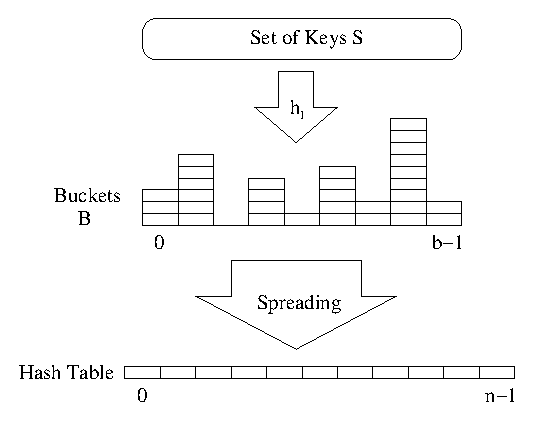
\includegraphics{figs/brz.ps}%
\end{picture}%
\setlength{\unitlength}{4144sp}%
%
\begingroup\makeatletter\ifx\SetFigFont\undefined%
\gdef\SetFigFont#1#2#3#4#5{%
  \reset@font\fontsize{#1}{#2pt}%
  \fontfamily{#3}\fontseries{#4}\fontshape{#5}%
  \selectfont}%
\fi\endgroup%
\begin{picture}(3704,2091)(1426,-5161)
\put(2570,-4301){\makebox(0,0)[lb]{\smash{{\SetFigFont{7}{8.4}{\familydefault}{\mddefault}{\updefault}0}}}}
\put(2782,-4301){\makebox(0,0)[lb]{\smash{{\SetFigFont{7}{8.4}{\familydefault}{\mddefault}{\updefault}1}}}}
\put(2996,-4301){\makebox(0,0)[lb]{\smash{{\SetFigFont{7}{8.4}{\familydefault}{\mddefault}{\updefault}2}}}}
\put(4060,-4006){\makebox(0,0)[lb]{\smash{{\SetFigFont{7}{8.4}{\familydefault}{\mddefault}{\updefault}Buckets}}}}
\put(3776,-4301){\makebox(0,0)[lb]{\smash{{\SetFigFont{7}{8.4}{\familydefault}{\mddefault}{\updefault}${\lceil n/b\rceil - 1}$}}}}
\put(4563,-3329){\makebox(0,0)[lb]{\smash{{\SetFigFont{7}{8.4}{\familydefault}{\mddefault}{\updefault}Key Set $S$}}}}
\put(2009,-3160){\makebox(0,0)[lb]{\smash{{\SetFigFont{7}{8.4}{\familydefault}{\mddefault}{\updefault}0}}}}
\put(2221,-3160){\makebox(0,0)[lb]{\smash{{\SetFigFont{7}{8.4}{\familydefault}{\mddefault}{\updefault}1}}}}
\put(4315,-3160){\makebox(0,0)[lb]{\smash{{\SetFigFont{7}{8.4}{\familydefault}{\mddefault}{\updefault}n-1}}}}
\put(1992,-5146){\makebox(0,0)[lb]{\smash{{\SetFigFont{7}{8.4}{\familydefault}{\mddefault}{\updefault}0}}}}
\put(2204,-5146){\makebox(0,0)[lb]{\smash{{\SetFigFont{7}{8.4}{\familydefault}{\mddefault}{\updefault}1}}}}
\put(4298,-5146){\makebox(0,0)[lb]{\smash{{\SetFigFont{7}{8.4}{\familydefault}{\mddefault}{\updefault}n-1}}}}
\put(4546,-4977){\makebox(0,0)[lb]{\smash{{\SetFigFont{7}{8.4}{\familydefault}{\mddefault}{\updefault}Hash Table}}}}
\put(1441,-3616){\makebox(0,0)[lb]{\smash{{\SetFigFont{7}{8.4}{\familydefault}{\mddefault}{\updefault}Partitioning}}}}
\put(1441,-4426){\makebox(0,0)[lb]{\smash{{\SetFigFont{7}{8.4}{\familydefault}{\mddefault}{\updefault}Searching}}}}
\put(1981,-4786){\makebox(0,0)[lb]{\smash{{\SetFigFont{5}{6.0}{\familydefault}{\mddefault}{\updefault}MPHF$_0$}}}}
\put(2521,-4786){\makebox(0,0)[lb]{\smash{{\SetFigFont{5}{6.0}{\familydefault}{\mddefault}{\updefault}MPHF$_1$}}}}
\put(3016,-4786){\makebox(0,0)[lb]{\smash{{\SetFigFont{5}{6.0}{\familydefault}{\mddefault}{\updefault}MPHF$_2$}}}}
\put(3826,-4786){\makebox(0,0)[lb]{\smash{{\SetFigFont{5}{6.0}{\familydefault}{\mddefault}{\updefault}MPHF$_{\lceil n/b \rceil - 1}$}}}}
\end{picture}%
\vspace{-1mm}
\caption{Main steps of our algorithm}
\label{fig:new-algo-main-steps}
\vspace{-3mm}
\end{figure}

The partitioning step takes a key set $S$ and uses a universal hash function 
$h_0$ proposed by Jenkins~\cite{j97} 
%for each key $k \in S$ of length $|k|$ 
to transform each key~$k\in S$ into an integer~$h_0(k)$.
Reducing~$h_0(k)$ modulo~$\lceil n/b\rceil$, we partition~$S$ into $\lceil n/b
\rceil$ buckets containing at most 256 keys in each bucket (with high
probability).  

The searching step generates a MPHF$_i$ for each bucket $i$, 
$0 \leq i < \lceil n/b \rceil$.
The resulting MPHF $h(k)$, $k \in S$, is given by
\begin{eqnarray}\label{eq:mphf}
h(k) = \mathrm{MPHF}_i (k) + \mathit{offset}[i], 
\end{eqnarray}
where~$i=h_0(k)\bmod\lceil n/b\rceil$.
The $i$th entry~$\mathit{offset}[i]$ of the displacement vector
$\mathit{offset}$, $0 \leq i < \lceil n/b \rceil$, contains the total number
of keys in the buckets from 0 to $i-1$, that is, it gives the interval of the
keys in the hash table addressed by the MPHF$_i$.  In the following we explain
each step in detail.




%% Nivio: 21/jan/06
% Time-stamp: <Monday 30 Jan 2006 03:57:28am EDT yoshi@ime.usp.br>
\vspace{-2mm}
\subsection{Partitioning step}
\label{sec:partitioning-keys}

The set $S$ of $n$ keys is partitioned into $\lceil n/b \rceil$ buckets, 
where $b$ is a suitable parameter chosen to guarantee
that each bucket has at most 256 keys with high probability
(see Section~\ref{sec:determining-b}).
The partitioning step works as follows:

\begin{figure}[h]
\hrule 
\hrule 
\vspace{2mm}
\begin{tabbing}
aa\=type booleanx \==  (false, true); \kill
\> $\blacktriangleright$ Let $\beta$ be the size in bytes of the set $S$ \\ 
\> $\blacktriangleright$ Let $\mu$ be the size in bytes of an a priori reserved \\
\> ~~~ internal memory area \\ 
\> $\blacktriangleright$ Let $N = \lceil \beta/\mu \rceil$ be the number of key blocks that will \\
\> ~~~ be read from disk into an internal memory area \\
\> $\blacktriangleright$ Let $\mathit{size}$ be a vector that stores the size of each bucket \\
\> $1.$ {\bf for} $j = 1$ {\bf to} $N$ {\bf do} \\
\> ~~ $1.1$ Read block $B_j$ of keys from disk \\
\> ~~ $1.2$ Cluster $B_j$ into $\lceil n/b \rceil$ buckets using a bucket sort \\
\> ~~~~~~~ algorithm and update the entries in the vector {\it size} \\
\> ~~ $1.3$ Dump $B_j$ to the disk into File $j$\\
\> $2.$ Compute the {\it offset} vector and dump it to the disk.
\end{tabbing}
\hrule 
\hrule 
\vspace{-1.0mm}
\caption{Partitioning step}
\vspace{-3mm}
\label{fig:partitioningstep}
\end{figure}

Statement 1.1 of the {\bf for} loop presented in Figure~\ref{fig:partitioningstep} 
reads sequentially all the keys of block $B_j$ from disk into an internal area
of size $\mu$.

Statement 1.2 performs an indirect bucket sort of the keys in block $B_j$
and at the same time updates the entries in the vector {\em size}.
Let us briefly describe how~$B_j$ is partitioned among the~$\lceil n/b\rceil$
buckets. 
We use a local array of $\lceil n/b \rceil$ counters to store a 
count of how many keys from $B_j$ belong to each bucket.
%At the same time, the global vector {\it size} is computed based on the local 
%counters. 
The pointers to the keys in each bucket $i$, $0 \leq i < \lceil n/b \rceil$,
are stored in contiguous positions in an array.
For this we first reserve the required number of entries
in this array of pointers using the information from the array of counters. 
Next, we place the pointers to the keys in each bucket into the respective
reserved areas in the array (i.e., we place the pointers to the keys in bucket 0, 
followed by the pointers to the keys in bucket 1, and so on).

\enlargethispage{2\baselineskip}
To find the bucket address of a given key
we use the universal hash function $h_0(k)$~\cite{j97}.
Key~$k$ goes into bucket~$i$, where
%Then, for each integer $h_0(k)$ the respective bucket address is obtained
%as follows:
\begin{eqnarray} \label{eq:bucketindex}
i=h_0(k) \bmod \left \lceil \frac{n}{b} \right \rceil.
\end{eqnarray}

Figure~\ref{fig:brz-partitioning}(a) shows a \emph{logical} view of the
$\lceil n/b \rceil$ buckets generated in the partitioning step.
%In this case, the keys of each bucket are put together by the pointers to
%each key stored 
%in contiguous positions in the array of pointers.
In reality, the keys belonging to each bucket are distributed among many files,
as depicted in Figure~\ref{fig:brz-partitioning}(b).
In the example of Figure~\ref{fig:brz-partitioning}(b), the keys in bucket 0 
appear in files 1 and $N$, the keys in bucket 1 appear in files 1, 2
and $N$, and so on. 

\vspace{-7mm}
\begin{figure}[ht]
\centering
\begin{picture}(0,0)%
\includegraphics{figs/brz-partitioning.ps}%
\end{picture}%
\setlength{\unitlength}{4144sp}%
%
\begingroup\makeatletter\ifx\SetFigFont\undefined%
\gdef\SetFigFont#1#2#3#4#5{%
  \reset@font\fontsize{#1}{#2pt}%
  \fontfamily{#3}\fontseries{#4}\fontshape{#5}%
  \selectfont}%
\fi\endgroup%
\begin{picture}(4371,1403)(1,-6977)
\put(333,-6421){\makebox(0,0)[lb]{\smash{{\SetFigFont{7}{8.4}{\familydefault}{\mddefault}{\updefault}0}}}}
\put(545,-6421){\makebox(0,0)[lb]{\smash{{\SetFigFont{7}{8.4}{\familydefault}{\mddefault}{\updefault}1}}}}
\put(759,-6421){\makebox(0,0)[lb]{\smash{{\SetFigFont{7}{8.4}{\familydefault}{\mddefault}{\updefault}2}}}}
\put(1539,-6421){\makebox(0,0)[lb]{\smash{{\SetFigFont{7}{8.4}{\familydefault}{\mddefault}{\updefault}${\lceil n/b\rceil - 1}$}}}}
\put(541,-6676){\makebox(0,0)[lb]{\smash{{\SetFigFont{7}{8.4}{\familydefault}{\mddefault}{\updefault}Buckets Logical View}}}}
\put(3547,-6120){\makebox(0,0)[lb]{\smash{{\SetFigFont{12}{14.4}{\familydefault}{\mddefault}{\updefault}.}}}}
\put(3547,-6188){\makebox(0,0)[lb]{\smash{{\SetFigFont{12}{14.4}{\familydefault}{\mddefault}{\updefault}.}}}}
\put(3547,-6255){\makebox(0,0)[lb]{\smash{{\SetFigFont{12}{14.4}{\familydefault}{\mddefault}{\updefault}.}}}}
\put(3107,-6120){\makebox(0,0)[lb]{\smash{{\SetFigFont{12}{14.4}{\familydefault}{\mddefault}{\updefault}.}}}}
\put(3107,-6188){\makebox(0,0)[lb]{\smash{{\SetFigFont{12}{14.4}{\familydefault}{\mddefault}{\updefault}.}}}}
\put(3107,-6255){\makebox(0,0)[lb]{\smash{{\SetFigFont{12}{14.4}{\familydefault}{\mddefault}{\updefault}.}}}}
\put(4177,-6224){\makebox(0,0)[lb]{\smash{{\SetFigFont{12}{14.4}{\familydefault}{\mddefault}{\updefault}.}}}}
\put(4177,-6269){\makebox(0,0)[lb]{\smash{{\SetFigFont{12}{14.4}{\familydefault}{\mddefault}{\updefault}.}}}}
\put(4177,-6314){\makebox(0,0)[lb]{\smash{{\SetFigFont{12}{14.4}{\familydefault}{\mddefault}{\updefault}.}}}}
\put(3016,-6721){\makebox(0,0)[lb]{\smash{{\SetFigFont{7}{8.4}{\familydefault}{\mddefault}{\updefault}File 1}}}}
\put(3466,-6721){\makebox(0,0)[lb]{\smash{{\SetFigFont{7}{8.4}{\familydefault}{\mddefault}{\updefault}File 2}}}}
\put(4096,-6721){\makebox(0,0)[lb]{\smash{{\SetFigFont{7}{8.4}{\familydefault}{\mddefault}{\updefault}File N}}}}
\put(3196,-6946){\makebox(0,0)[lb]{\smash{{\SetFigFont{7}{8.4}{\familydefault}{\mddefault}{\updefault}Buckets Physical View}}}}
\end{picture}%
\caption{Situation of the buckets at the end of the partitioning step: (a) Logical view (b) Physical view}
\label{fig:brz-partitioning}
\vspace{-2mm}
\end{figure}

This scattering of the keys in the buckets could generate a performance
problem because of the potential number of seeks  
needed to read the keys in each bucket from the $N$ files in disk 
during the searching step. 
But, as we show later in Section~\ref{sec:analytcal-results}, the number of seeks 
can be kept small using buffering techniques.
Considering that only the vector {\it size}, which has $\lceil n/b \rceil$
one-byte entries (remember that each bucket has at most 256 keys),
must be maintained in main memory during the searching step,
almost all main memory is available to be used as disk I/O buffer.

The last step is to compute the {\it offset} vector and dump it to the disk.
We use the vector $\mathit{size}$ to compute the
$\mathit{offset}$ displacement vector. 
The $\mathit{offset}[i]$ entry contains the number of keys 
in the buckets $0, 1, \dots, i-1$.
As {\it size}$[i]$ stores the number of keys
in bucket $i$, where $0 \leq i <\lceil n/b \rceil$, we have
\begin{displaymath}
\mathit{offset}[i] = \sum_{j=0}^{i-1} \mathit{size}[j] \cdot
\end{displaymath}
 

%% Nivio: 22/jan/06
% Time-stamp: <Monday 30 Jan 2006 03:57:35am EDT yoshi@ime.usp.br>
\vspace{-7mm}
\subsection{Searching step}
\label{sec:searching}

\enlargethispage{2\baselineskip}
The searching step is responsible for generating a MPHF for each 
bucket.
Figure~\ref{fig:searchingstep} presents the searching step algorithm.
\vspace{-2mm}
\begin{figure}[h]
%\centering
\hrule 
\hrule 
\vspace{2mm}
\begin{tabbing}
aa\=type booleanx \==  (false, true); \kill
\> $\blacktriangleright$ Let $H$ be a minimum heap of size $N$, where the \\
\> ~~ order relation in $H$ is given by Eq.~(\ref{eq:bucketindex}), that is, the\\
\> ~~ remove operation removes the item with smallest $i$\\ 
\> $1.$ {\bf for} $j = 1$ {\bf to} $N$ {\bf do} \{ Heap construction \}\\
\> ~~ $1.1$ Read key $k$ from File $j$ on disk\\
\> ~~ $1.2$ Insert $(i, j, k)$ in $H$ \\
\> $2.$ {\bf for} $i = 0$ {\bf to} $\lceil n/b \rceil - 1$ {\bf do} \\
\> ~~ $2.1$ Read bucket $i$ from disk driven by heap $H$ \\
\> ~~ $2.2$ Generate a MPHF for bucket $i$ \\
\> ~~ $2.3$ Write the description of MPHF$_i$ to the disk 
\end{tabbing}
\vspace{-1mm}
\hrule 
\hrule 
\caption{Searching step}
\label{fig:searchingstep}
\vspace{-4mm}
\end{figure}

Statement 1 of Figure~\ref{fig:searchingstep} inserts one key from each file
in a minimum heap $H$ of size $N$.
The order relation in $H$ is given by the bucket address $i$ given by
Eq.~(\ref{eq:bucketindex}).

%\enlargethispage{-\baselineskip}
Statement 2 has two important steps.
In statement 2.1, a bucket is read from disk,
as described below.
%in Section~\ref{sec:readingbucket}. 
In statement 2.2, a MPHF is generated for each bucket $i$, as described 
in the following.
%in Section~\ref{sec:mphfbucket}.
The description of MPHF$_i$ is a vector $g_i$ of 8-bit integers.
Finally, statement 2.3 writes the description $g_i$ of MPHF$_i$ to disk.

\vspace{-3mm}
\label{sec:readingbucket}
\subsubsection{Reading a bucket from disk.} 

In this section we present the refinement of statement 2.1 of
Figure~\ref{fig:searchingstep}.
The algorithm to read bucket $i$ from disk is presented 
in Figure~\ref{fig:readingbucket}.

\begin{figure}[h]
\hrule 
\hrule 
\vspace{2mm}
\begin{tabbing}
aa\=type booleanx \==  (false, true); \kill
\> $1.$ {\bf while} bucket $i$ is not full {\bf do} \\
\> ~~ $1.1$ Remove $(i, j, k)$ from $H$\\
\> ~~ $1.2$ Insert $k$ into bucket $i$ \\
\> ~~ $1.3$ Read sequentially all keys $k$ from File $j$ that have \\
\> ~~~~~~~ the same $i$ and insert them into bucket $i$ \\
\> ~~ $1.4$ Insert the triple $(i, j, x)$ in $H$, where $x$ is the first \\
\> ~~~~~~~ key read from File $j$ that does not have the \\ 
\> ~~~~~~~ same bucket index $i$
\end{tabbing}
\hrule 
\hrule 
\vspace{-1.0mm}
\caption{Reading a bucket}
\vspace{-4.0mm}
\label{fig:readingbucket}
\end{figure}

Bucket $i$ is distributed among many files and the heap $H$ is used to drive a
multiway merge operation.
In Figure~\ref{fig:readingbucket}, statement 1.1 extracts and removes triple 
$(i, j, k)$ from $H$, where $i$ is a minimum value in $H$.
Statement 1.2 inserts key $k$ in bucket $i$.
Notice that the $k$ in the triple $(i, j, k)$ is in fact a pointer to
the first byte of the key that is kept in contiguous positions of an array of characters
(this array containing the keys is initialized during the heap construction
in statement 1 of Figure~\ref{fig:searchingstep}).
Statement 1.3 performs a seek operation in File $j$ on disk for the first 
read operation and reads sequentially all keys $k$ that have the same $i$ 
%(obtained from Eq.~(\ref{eq:bucketindex})) 
and inserts them all in bucket $i$.
Finally, statement 1.4 inserts in $H$ the triple $(i, j, x)$,  
where $x$ is the first key read from File $j$ (in statement 1.3) 
that does not have the same bucket address as the previous keys.

The number of seek operations on disk performed in statement 1.3 is discussed
in Section~\ref{sec:linearcomplexity}, 
where we present a buffering technique that brings down 
the time spent with seeks.

\vspace{-2mm}
\enlargethispage{2\baselineskip}
\subsubsection{Generating a MPHF for each bucket.} \label{sec:mphfbucket}

To the best of our knowledge the algorithm we have designed in
our previous work~\cite{bkz05} is the fastest published algorithm for
constructing MPHFs.
That is why we are using that algorithm as a building block for the 
algorithm presented here.

%\enlargethispage{-\baselineskip}
Our previous algorithm is a three-step internal memory based algorithm
that produces a MPHF based on random graphs.
For a set of $n$ keys, the algorithm outputs the resulting MPHF in expected time $O(n)$.
For a given bucket $i$, $0 \leq i < \lceil n/b \rceil$, the corresponding MPHF$_i$ 
has the following form:
\begin{eqnarray}
        \mathrm{MPHF}_i(k) &=& g_i[a] + g_i[b] \label{eq:mphfi}
\end{eqnarray} 
where $a = h_{i1}(k) \bmod t$, $b = h_{i2}(k) \bmod t$ and
$t = c\times \mathit{size}[i]$. The functions
$h_{i1}(k)$ and $h_{i2}(k)$ are the same universal function proposed by Jenkins~\cite{j97}
that was used in the partitioning step described in Section~\ref{sec:partitioning-keys}.

In order to generate the function above the algorithm involves the generation of simple random graphs
$G_i = (V_i, E_i)$ with~$|V_i|=t=c\times\mathit{size}[i]$ and $|E_i|=\mathit{size}[i]$, with  $c \in [0.93, 1.15]$.
To generate a simple random graph with high 
probability\footnote{We use the terms `with high probability'
to mean `with probability tending to~$1$ as~$n\to\infty$'.}, two vertices $a$ and $b$ are
computed for each key $k$ in bucket $i$.
Thus, each bucket $i$ has a corresponding graph~$G_i=(V_i,E_i)$, where $V_i=\{0,1,
\ldots,t-1\}$ and $E_i=\big\{\{a,b\}:k \in \mathrm{bucket}\: i\big\}$.
In order to get a simple graph, 
the algorithm repeatedly selects $h_{i1}$ and $h_{i2}$ from a family of universal hash functions
until the corresponding graph is simple.
The probability of getting a simple graph is $p=e^{-1/c^2}$.
For $c=1$, this probability is $p \simeq 0.368$, and the expected number of 
iterations to obtain a simple graph is~$1/p \simeq 2.72$.

The construction of MPHF$_i$ ends with a computation of a suitable labelling of the vertices
of~$G_i$. The labelling is stored into vector $g_i$.
We choose~$g_i[v]$ for each~$v\in V_i$ in such
a way that Eq.~(\ref{eq:mphfi}) is a MPHF for bucket $i$.
In order to get the values of each entry of $g_i$ we first 
run a breadth-first search on the 2-\textit{core} of $G_i$, i.e., the maximal subgraph 
of~$G_i$ with minimal degree at least~$2$ (see, e.g., \cite{b01,jlr00,pw04}) and
a depth-first search on the acyclic part of $G_i$ (see \cite{bkz05} for details).


%\input{computingoffset}
%\input{hashingbuckets}
% Nivio: 29/jan/06
% Time-stamp: <Monday 30 Jan 2006 04:01:40am EDT yoshi@ime.usp.br>
\enlargethispage{2\baselineskip}
\subsection{Determining~$b$}
\label{sec:determining-b}
\begin{table*}[t]
\begin{center}
{\small %\scriptsize
\begin{tabular}{|c|ccc|ccc|}
\hline
\raisebox{-0.7em}{$n$} & \multicolumn{3}{c|}{\raisebox{-1mm}{b=128}}  &
\multicolumn{3}{c|}{\raisebox{-1mm}{b=175}}\\
\cline{2-4} \cline{5-7}
 & \raisebox{-0.5mm}{Worst Case} & \raisebox{-0.5mm}{Average} &\raisebox{-0.5mm}{Eq.~(\ref{eq:maxbs})} 
 & \raisebox{-0.5mm}{Worst Case} & \raisebox{-0.5mm}{Average} &\raisebox{-0.5mm}{Eq.~(\ref{eq:maxbs})} \\
\hline
$1.0 \times 10^6$  & 177 & 172.0 & 176  & 232 & 226.6 & 230 \\
%$2.0 \times 10^6$  & 179 & 174.0 & 178  & 236 & 228.5 & 232 \\
$4.0 \times 10^6$  & 182 & 177.5 & 179  & 241 & 231.8 & 234 \\
%$8.0 \times 10^6$  & 186 & 181.6 & 181  & 238 & 234.2 & 236 \\
$1.6 \times 10^7$  & 184 & 181.6 & 183  & 241 & 236.1 & 238 \\
%$3.2 \times 10^7$  & 191 & 183.9 & 184  & 240 & 236.6 & 240 \\
$6.4 \times 10^7$  & 195 & 185.2 & 186  & 244 & 239.0 & 242 \\
%$1.28 \times 10^8$ & 193 & 187.7 & 187  & 244 & 239.7 & 244 \\
$5.12 \times 10^8$ & 196 & 191.7 & 190  & 251 & 246.3 & 247 \\
$1.0 \times 10^9$  & 197 & 191.6 & 192  & 253 & 248.9 & 249 \\
\hline
\end{tabular}
\vspace{-1mm}
}
\end{center}
\caption{Values for $\mathit{BS}_{\mathit{max}}$: worst case and average case obtained in the experiments and using Eq.~(\ref{eq:maxbs}), 
considering $b=128$ and $b=175$ for different number $n$ of keys in $S$.} 
\label{tab:comparison}
\vspace{-6mm}
\end{table*}

The partitioning step can be viewed as the well known ``balls into bins'' 
problem~\cite{ra98,dfm02} where~$n$ keys (the balls) are placed independently and 
uniformly into $\lceil n/b\rceil$ buckets (the bins). The main question related to that problem we are interested 
in is: what is the maximum number of keys in any bucket? 
In fact, we want to get the maximum value for $b$ that makes the maximum number of keys in any bucket
no greater than 256 with high probability. 
This is important, as we wish to use 8 bits per entry in the vector $g_i$ of
each $\mathrm{MPHF}_i$, 
where $0 \leq i < \lceil n/b\rceil$.      
Let $\mathit{BS}_{\mathit{max}}$ be the maximum number of keys in any bucket.

Clearly, $\BSmax$ is the maximum
of~$\lceil n/b\rceil$ random variables~$Z_i$, each with binomial
distribution~$\Bi(n,p)$ with parameters~$n$ and~$p=1/\lceil n/b\rceil$.
However, the~$Z_i$ are not independent.  Note that~$\Bi(n,p)$ has mean and
variance~$\simeq b$.  To give an upper estimate for the probability of the
event~$\BSmax\geq \gamma$, we can estimate the probability that we have~$Z_i\geq \gamma$
for a fixed~$i$, and then sum these estimates over all~$i$.
Let~$\gamma=b+\sigma\sqrt{b\ln(n/b)}$, where~$\sigma=\sqrt2$.
Approximating~$\Bi(n,p)$ by the normal distribution with mean and
variance~$b$, we obtain the
estimate~$(\sigma\sqrt{2\pi\ln(n/b)})^{-1}\times\exp(-(1/2)\sigma^2\ln(n/b))$ for
the probability that~$Z_i\geq \gamma$ occurs, which, summed over all~$i$, gives
that the probability that~$\BSmax\geq \gamma$ occurs is at
most~$1/(\sigma\sqrt{2\pi\ln(n/b)})$, which tends to~$0$ as~$n\to\infty$.
Thus, we have shown that, with high probability, 
\begin{equation}
  \label{eq:maxbs}
  \BSmax\leq b+\sqrt{2b\ln{n\over b}}.
\end{equation}

% The traditional approach used to estimate $\mathit{BS}_{\mathit{max}}$ with high probability is 
% to consider $\mathit{BS}_{\mathit{max}}$ as a random variable that follows a binomial distribution 
% that can be approximated by a poisson distribution. This yields a good approximation
% when the number of balls is lower than or equal to the number of bins~\cite{g81}. In our case,
% the number of balls is greater than the number of buckets.
% % and that is why we have used more recent works to estimate $\mathit{BS}_{\mathit{max}}$. 
% As $b > \ln (n/b)$, we can use the result by Raab and Steger~\cite{ra98} to estimate
% $\mathit{BS}_{\mathit{max}}$ with high probability. 
% The following equation gives the estimation, where $\sigma=\sqrt{2}$:  
% \begin{eqnarray} \label{eq:maxbs}
% \mathit{BS}_{\mathit{max}} = b + O \left( \sqrt{b\ln\frac{n}{b}} \right) = b + \sigma \times \left(\sqrt{b\ln\frac{n}{b}} \right)
% \end{eqnarray}

% In order to estimate the suitable constant $\sigma$ we did a linear 
% regression suppressing the constant term. 
% We use the equation $BS_{max} - b = \sigma \times \sqrt{b\ln (n/b)}$ 
% in the linear regression considering $y=BS_{max} - b$ and $x=\sqrt{b\ln (n/b)}$. 
% In order to obtain data to be used in the linear regression we set 
% b=128 and ran the new algorithm ten times 
% for n equal to 1, 2, 4, 8, 16, 32, 64, 128, 512, 1000 million keys.  
% Taking a confidence level equal to 95\% we got 
% $\sigma = 2.11 \pm 0.03$. 
% The coefficient of determination was $99.6\%$, which means that the linear 
% regression explains $99.6\%$ of the data variation and only $0.4\%$ 
% is due to experimental errors.
% Therefore, Eq.~(\ref{eq:maxbs}) with $\sigma = 2.11 \pm 0.03$ and $b=128$ 
% makes a very good estimation of the maximum number of keys in any bucket.

% Repeating the same experiments for $b$ equals to $175$ and  
% a confidence level of $95\%$ we got $\sigma = 2.07 \pm 0.03$.
% Again we verified that Eq.~(\ref{eq:maxbs}) with $\sigma = 2.07 \pm 0.03$ and $b=175$ is 
% a very good estimation of the maximum number of keys in any bucket once the
% coefficient of determination obtained was $99.7 \%$ and $\sigma$ is in a very narrow range.

In our algorithm the maximum number of keys in any bucket must be at most 256. 
Table~\ref{tab:comparison} presents the values for $\mathit{BS}_{\mathit{max}}$
obtained experimentally and using Eq.~(\ref{eq:maxbs}).
The table presents the worst case and the average case, 
considering $b=128$,  $b=175$ and Eq.~(\ref{eq:maxbs}),
for several numbers~$n$ of keys in $S$. 
The estimation given by Eq.~(\ref{eq:maxbs}) is very close to the experimental
results.

Now we estimate the biggest problem our algorithm is able to solve for 
a given $b$. 
Using Eq.~(\ref{eq:maxbs}) considering $b=128$, $b=175$ and imposing
that~$\mathit{BS}_{\mathit{max}}\leq256$, 
the sizes of the biggest key set our algorithm 
can deal with are $10^{30}$ keys and $10^{10}$ keys, respectively. 
%It is also important to have $b$ as big as possible, once its value is
%related to the space required to store the resultant MPHF, as shown later on.
%Table~\ref{tab:bp} shows the biggest problem the algorithm can solve.
% The values were obtained from Eq.~(\ref{eq:maxbs}), 
% considering $b=128$ and~$b=175$ and imposing
% that~$\mathit{BS}_{\mathit{max}}\leq256$. 

% We set $\sigma=2.14$ because it was the greatest value obtained for $\sigma$
% in the two linear regression we did.
% \vspace{-3mm} 
% \begin{table}[htb]
% \begin{center}
% {\small %\scriptsize
% \begin{tabular}{|c|c|}
% \hline
% b    & Problem size ($n$) \\
% \hline
% 128  & $10^{30}$ keys  \\
% 175  & $10^{10}$ keys  \\
% \hline
% \end{tabular}
% \vspace{-1mm}
% }
% \end{center}
% \caption{Using Eq.~(\ref{eq:maxbs}) to estimate the biggest problem our algorithm can solve.}
% %considering $\sigma=\sqrt{2}$.}
% \label{tab:bp}
% \vspace{-14mm}
% \end{table}

%\input{analyticalandexperimentalresults}
%% Nivio: 23/jan/06 29/jan/06
% Time-stamp: <Monday 30 Jan 2006 03:56:47am EDT yoshi@ime.usp.br>
\enlargethispage{2\baselineskip}
\section{Analytical results}
\label{sec:analytcal-results}

\vspace{-1mm}
The purpose of this section is fourfold.
First, we show that our algorithm runs in expected time $O(n)$. 
Second, we present the main memory requirements for constructing the MPHF.
Third, we discuss the cost of evaluating the resulting MPHF.
Fourth, we present the space required to store the resulting MPHF.

\vspace{-2mm}
\subsection{The linear time complexity}
\label{sec:linearcomplexity}
 
First, we show that the partitioning step presented in
Figure~\ref{fig:partitioningstep} runs in $O(n)$ time.
Each iteration of the {\bf for} loop in statement~1
runs in $O(|B_j|)$ time, $1 \leq j \leq N$, where $|B_j|$ is the 
number of keys 
that fit in block $B_j$ of size $\mu$. This is because statement 1.1 just reads
$|B_j|$ keys from disk, statement 1.2 runs a bucket sort like algorithm 
that is well known to be linear in the number of keys it sorts (i.e., $|B_j|$ keys),
and statement 1.3 just dumps $|B_j|$ keys to the disk into File $j$.
Thus, the {\bf for} loop runs in $O(\sum_{j=1}^{N}|B_j|)$ time. 
As $\sum_{j=1}^{N}|B_j|=n$, then the partitioning step runs in $O(n)$ time.

Second, we show that the searching step presented in 
Figure~\ref{fig:searchingstep} also runs in $O(n)$ time.
The heap construction in statement 1 runs in $O(N)$ time, for $N \ll n$.
We have assumed that insertions and deletions in the heap cost $O(1)$ because 
$N$ is typically much smaller than $n$ (see \cite[Section 6.4]{bkz06t} for details).
Statement 2 runs in $O(\sum_{i=0}^{\lceil n/b \rceil - 1} \mathit{size}[i])$ time
(remember that $\mathit{size}[i]$ stores the number of keys in bucket $i$).
As $\sum_{i=0}^{\lceil n/b \rceil - 1} \mathit{size}[i] = n$, if 
statements 2.1, 2.2 and 2.3 run in $O(\mathit{size}[i])$ time, then statement 2
runs in $O(n)$ time.

%Statement 2.1 runs the algorithm to read a bucket from disk. That algorithm reads $\mathit{size}[i]$
%keys of bucket $i$ that might be spread into many files or, in the worst case,
%into $|BS_{max}|$ files, where $|BS_{max}|$ is the number of keys in the bucket of maximum size.
%It uses the heap $H$ to drive a multiway merge of the sprayed bucket $i$. 
%As we are considering that each read/write on disk costs $O(1)$ and
%each heap operation also costs $O(1)$ (recall $N \ll n$), then  statement 2.1
%costs $O(\mathit{size}[i])$ time.
%We need to take into account that this step could generate a lot of seeks on disk. 
%However, the number of seeks can be amortized (see Section~\ref{sec:contr-disk-access})
%and that is why we have been able of getting a MPHF for a set of 1 billion keys in less 
%than 4 hours using a machine with just 500 MB of main memory
%(see Section~\ref{sec:performance}).
Statement 2.1 reads $O(\mathit{size}[i])$ keys of bucket $i$
and is detailed in Figure~\ref{fig:readingbucket}.
As we are assuming that each read or write on disk costs $O(1)$ and
each heap operation also costs $O(1)$, statement~2.1
takes $O(\mathit{size}[i])$ time.
However, the keys of bucket $i$ are distributed in at most~$BS_{max}$ files on disk 
in the worst case
(recall that $BS_{max}$ is the maximum number of keys found in any bucket).
Therefore, we need to take into account that 
the critical step in reading a bucket is in statement~1.3 of Figure~\ref{fig:readingbucket},
where a seek operation in File $j$
may be performed by the first read operation.

In order to amortize the number of seeks performed we use a buffering technique~\cite{k73}.
We create a buffer $j$ of size \textbaht$\: = \mu/N$ for each file $j$, 
where $1\leq j \leq N$
(recall that $\mu$ is the size in bytes of an a priori reserved internal memory area).
Every time a read operation is requested to file $j$ and the data is not found 
in the $j$th~buffer, \textbaht~bytes are read from file $j$ to buffer $j$. 
Hence, the number of seeks performed in the worst case is given by
$\beta/$\textbaht~(remember that $\beta$ is the size in bytes of $S$).
For that we have made the pessimistic assumption that one seek happens every time 
buffer $j$ is filled in. 
Thus, the number of seeks performed in the worst case is $64n/$\textbaht, since
each URL is 64 bytes long on average. Therefore, the number of seeks is linear on 
$n$ and amortized by \textbaht.

It is important to emphasize two things.
First, the operating system uses techniques
to diminish the number of seeks and the average seek time. 
This makes the amortization factor to be greater than \textbaht~in practice.  
Second, almost all main memory is available to be used as
file buffers because just a small vector
of $\lceil n/b\rceil$ one-byte entries must be maintained in main memory, 
as we show in Section~\ref{sec:memconstruction}.


Statement 2.2 runs our internal memory based algorithm in order to generate a MPHF for each bucket.
That algorithm is linear, as we showed in~\cite{bkz05}. As it is applied to buckets with {\it size}$[i]$ keys, statement~2.2 takes $O(\mathit{size}[i])$ time.

Statement 2.3 has time complexity $O(\mathit{size}[i])$ because it writes to disk 
the description of each generated MPHF and each description is stored in
$c \times \mathit{size}[i] + O(1)$ bytes, where $c\in[0.93,1.15]$.
In conclusion, our algorithm takes $O(n)$ time because both the partitioning and
the searching steps run in $O(n)$ time. 

An experimental validation of the above proof and a performance comparison with 
our internal memory based algorithm~\cite{bkz05} were not included here due to 
space restrictions but can be found in~\cite{bkz06t} and also in the appendix.

\vspace{-1mm}
\enlargethispage{2\baselineskip}
\subsection{Space used for constructing a MPHF} 
\label{sec:memconstruction}

The vector {\it size} is kept in main memory 
all the time. 
The vector {\it size} has $\lceil n/b \rceil$ one-byte entries.
It stores the number of keys in each bucket and 
those values are less than or equal to 256. 
For example, for a set of 1 billion keys and $b=175$ the vector size needs 
$5.45$ megabytes of main memory.

We need an internal memory area of size $\mu$ bytes to be used in
the partitioning step and in the searching step. 
The size $\mu$ is fixed a priori and depends only on the amount 
of internal memory available to run the algorithm
(i.e., it does not depend on the size $n$ of the problem).

% One could argue about the a priori reserved internal memory area and the main memory
% required to run the indirect bucket sort algorithm.
% Those internal memory requirements do not depend on the size of the problem
% (i.e., the number of keys being hashed) and can be fixed a priori.

The additional space required in the searching step
is constant, once the problem was broken down
into several small problems (at most 256 keys) and 
the heap size is supposed to be much smaller than $n$ ($N \ll n$).
For example, for a set of 1 billion keys and an internal area of~$\mu = 250$ megabytes,
the number of files is $N = 248$. 

\vspace{-1mm}
\subsection{Evaluation cost of the MPHF} 

Now we consider the amount of CPU time 
required by the resulting MPHF at retrieval time.
The MPHF requires for each key the computation of three 
universal hash functions and three memory accesses 
(see Eqs.~(\ref{eq:mphf}), (\ref{eq:bucketindex}) and (\ref{eq:mphfi})).
This is not optimal. Pagh~\cite{p99} showed that any MPHF requires 
at least the computation of two universal hash functions and one memory
access.

\subsection{Description size of the MPHF} 

The number of bits required to store the MPHF generated by the algorithm 
is computed by Eq.~(\ref{eq:newmphfbits}). 
We need to store each $g_i$ vector presented in Eq.~(\ref{eq:mphfi}), where
$0\leq i < \lceil n/b \rceil$. As each bucket has at most 256 keys, each 
entry in a $g_i$ vector has 8~bits.  In each $g_i$ vector there are 
$c \times \mathit{size}[i]$ entries (recall $c\in[0.93, 1.15]$).
When we sum up the number of entries of $\lceil n/b \rceil$ $g_i$ vectors we have
$c\sum_{i=0}^{\lceil n/b \rceil -1} \mathit{size}[i]=cn$ entries.  We also need to
store $3 \lceil n/b \rceil$ integer numbers of 
$\log_2n$ bits referring respectively to the {\it offset} vector and the two random seeds of
$h_{1i}$ and $h_{2i}$. In addition, we need to store $\lceil n/b \rceil$ 8-bit entries of 
the vector {\it size}.  Therefore, 
\begin{eqnarray}\label{eq:newmphfbits}
\mathrm{Required\: Space} = 8cn + \frac{n}{b}\left( 3\log_2n +8\right) \:
\mathrm{bits}. 
\end{eqnarray}

Considering $c=0.93$ and $b=175$, the number of bits per key to store 
the description of the resulting MPHF for a set of 1~billion keys is $8.1$.
If we set $b=128$, then the bits per key ratio increases to $8.3$.
Theoretically, the number of bits required to store the MPHF in
Eq.~(\ref{eq:newmphfbits}) 
is $O(n\log n)$ as~$n\to\infty$. However, for sets of size up to $2^{b/3}$ keys 
the number of bits per key is lower than 9~bits (note that
$2^{b/3}>2^{58}>10^{17}$ for $b=175$).  
%For $b=175$, the number of bits per key will be close to 9 for a set of $2^{58}$ keys. 
Thus, in practice the resulting function is stored in $O(n)$ bits.

%\input{results}
% Time-stamp: <Monday 30 Jan 2006 12:38:06am EST yoshi@flare>
\enlargethispage{2\baselineskip}
\section{Concluding remarks}
\label{sec:concuding-remarks}

This paper has presented a novel external memory based algorithm for
constructing MPHFs that works for sets in the order of billions of keys.  The
algorithm outputs the resulting function in~$O(n)$ time and, furthermore, it
can be tuned to run only $34\%$ slower (see \cite{bkz06t} for details) than the fastest 
algorithm available in the literature for constructing MPHFs~\cite{bkz05}.  
In addition, the space
requirement of the resulting MPHF is of up to 9 bits per key for datasets of
up to $2^{58}\simeq10^{17.4}$ keys. 
 
The algorithm is simple and needs just a
small vector of size approximately 5.45 megabytes in main memory to construct
a MPHF for a collection of 1 billion URLs, each one 64 bytes long on average.
Therefore, almost all main memory is available to be used as disk I/O buffer.
Making use of such a buffering scheme considering an internal memory area of size
$\mu=200$ megabytes, our algorithm can produce a MPHF for a
set of 1 billion URLs in approximately 3.6 hours using a commodity PC of 2.4 gigahertz and
500 megabytes of main memory.  
If we increase both the main memory
available to 1 gigabyte and the internal memory area to $\mu=500$ megabytes, 
a MPHF for the set of 1 billion URLs is produced in approximately 3 hours. For any
key, the evaluation of the resulting MPHF takes three memory accesses and the
computation of three universal hash functions. 

In order to allow the reproduction of our results and the utilization of both the internal memory
based algorithm and the external memory based algorithm,
the algorithms are available at \texttt{http://cmph.sf.net}
under the GNU Lesser General Public License (LGPL).
They were implemented in the C language.

In future work, we will exploit the fact that the searching step intrinsically
presents a high degree of parallelism and requires $73\%$ of the
construction time.  Therefore, a parallel implementation of our algorithm will
allow the construction and the evaluation of the resulting function in parallel.
Therefore, the description of the resulting MPHFs will be distributed in the paralell 
computer allowing the scalability to sets of hundreds of billions of keys. 
This is an important contribution, mainly for applications related to the Web, as 
mentioned in Section~\ref{sec:intro}.




%\section{Acknowledgments}
This section is optional; it is a location for you
to acknowledge grants, funding, editing assistance and
what have you.  In the present case, for example, the
authors would like to thank Gerald Murray of ACM for
his help in codifying this \textit{Author's Guide}
and the \textbf{.cls} and \textbf{.tex} files that it describes.

%\begin{acknowledgements}
%If you'd like to thank anyone, place your comments here
%and remove the percent signs.
%\end{acknowledgements}

% BibTeX users please use
%\bibliographystyle{spmpsci}
%\bibliography{}   % name your BibTeX data base
\bibliographystyle{plain}
\bibliography{references}
\appendix
\section{Experimental Results}

% We now present some experimental results.
% The same experiments were run with our algorithm and
% the algorithm due to Czech, Havas and Majewski~\cite{chm92}, referred to as
% the CHM algorithm.
% The two algorithms were implemented in the C language and
% are available at \texttt{http://cmph.sf.net}.
% Our data consists
% of a collection of 100 million
% universe resource locations (URLs) collected from the Web.
% The average length of a URL in the collection is 63 bytes.
% All experiments were carried out on
% a computer running the Linux operating system, version 2.6.7,
% with a 2.4 gigahertz processor and
% 4 gigabytes of main memory.
% 
% Table~\ref{tab:characteristics} presents the main characteristics
% of the two algorithms.
% The number of edges in the graph $G=(V,E)$ is~$|S|=n$,
% the number of keys in the input set~$S$.
% The number of vertices of $G$ is equal to $1.15n$ and $2.09n$
% for our algorithm and the CHM algorithm, respectively.
% This measure is related to the amount of space to store the array $g$.
% This improves the space required to store a function in our algorithm to
% $55\%$ of the space required by the CHM algorithm.
% The number of critical edges
% is $\frac{1}{2}|E(G)|$ and 0 for our algorithm and the CHM algorithm,
% respectively.
% Our algorithm generates random graphs that contain cycles with high
% probability and the
% CHM algorithm
% generates
% acyclic random graphs.
% Finally, the CHM algorithm generates order preserving functions
% while our algorithm does not preserve order.
% 
% \vspace{-10pt}
% \begin{table}[htb]
% {\footnotesize 
% \begin{center}
% \begin{tabular}{|c|c|c|c|c|c|c|}
% \hline
%                  & $c$  & $|E(G)|$ & $|V(G)|=|g|$ & $|E(G_\crit)|$ & $G$     & Order preserving \\
% \hline
% Our  algorithm   & 1.15 & $n$      & $cn$         & $0.5|E(G)|$    & cyclic  & no \\
% \hline
% CHM  algorithm   & 2.09 & $n$      & $cn$         & 0              & acyclic & yes \\
% \hline
% \end{tabular}
% \end{center}
% }
% \caption{Main characteristics of the algorithms}
% \vspace{-25pt}
% \label{tab:characteristics}
% \end{table}
% 
% Table~\ref{tab:timeresults} presents time measurements.
% All times are in seconds.
% The table entries are averages over 50 trials.
% The column labelled $N_i$ gives
% the number of iterations to generate the random graph $G$
% in the mapping step of the algorithms.
% The next columns give the running times
% for the mapping plus ordering steps together and the searching
% step for each algorithm.
% The last column gives the percentage gain of our algorithm
% over the CHM algorithm.
% 
% \begin{table*}
% {\footnotesize 
% \begin{center}
% \begin{tabular}{|c|cccc|cccc|c|}
% \hline 
% \raisebox{-0.7em}{$n$} & \multicolumn{4}{c|}{\raisebox{-1mm}{Our algorithm}} &
% \multicolumn{4}{c|}{\raisebox{-1mm}{CHM algorithm}}& \raisebox{-0.2em}{Gain}\\
% \cline{2-5} \cline{6-9} 
%  & \raisebox{-1mm}{$N_i$} &\raisebox{-1mm}{Map+Ord} &
% \raisebox{-1mm}{Search} &\raisebox{-1mm}{Total}  &
% \raisebox{-1mm}{$N_i$} &\raisebox{-1mm}{Map+Ord} &\raisebox{-1mm}{Search} &
% \raisebox{-1mm}{Total} & \raisebox{0.2em}{(\%)}\\
% \hline
% %1,562,500    & 2.28 & 8.54   & 2.37   & 10.91   & 2.70 & 14.56    & 1.57   & 16.13    & 48 \\ %[1mm]
% %3,125,000    & 2.16 & 15.92  & 4.88   & 20.80   & 2.85 & 30.36    & 3.20   & 33.56    & 61 \\ %[1mm]
% 6,250,000    & 2.20 & 33.09  & 10.48  & 43.57   & 2.90 & 62.26    & 6.76   & 69.02    & 58 \\ %[1mm]
% 12,500,000   & 2.00 & 63.26  & 23.04  & 86.30   & 2.60 & 117.99   & 14.94  & 132.92   & 54 \\ %[1mm]
% 25,000,000   & 2.00 & 130.79 & 51.55  & 182.34  & 2.80 & 262.05   & 33.68  & 295.73   & 62 \\ %[1mm]
% %50,000,000   & 2.07 & 273.75 & 114.12 & 387.87  & 2.90 & 577.59   & 73.97  & 651.56   & 68 \\ %[1mm]
% 100,000,000  & 2.07 & 567.47 & 243.13 & 810.60  & 2.80 & 1,131.06 & 157.23 & 1,288.29 & 59 \\ %[1mm]
% \hline
% \end{tabular}
% \end{center}
% \caption{Time measurements
% for our algorithm and the CHM algorithm}
% \vspace{-25pt}
% \label{tab:timeresults}
% }\end{table*}
% 
% \enlargethispage{\baselineskip}
% The mapping step of the new algorithm is faster because
% the expected number of iterations in the mapping step to generate
% $G$ are 2.13 and 2.92 for our algorithm and the CHM algorithm, respectively.
% The graph $G$ generated by our algorithm
% has $1.15n$ vertices, against $2.09n$ for the CHM algorithm.
% These two facts make our algorithm faster in the mapping step.
% The ordering step of our algorithm is approximately equal to
% the time to check if $G$ is acyclic for the CHM algorithm.
% The searching step of the CHM algorithm is faster, but the total
% time of our algorithm is, on average, approximately 58\% faster
% than the CHM algorithm.
% 
% The experimental results fully backs the theoretical results.
% It is important to notice the times for the searching step:
% for both algorithms they are not the dominant times,
% and the experimental results clearly show
% a linear behavior for the searching step.
% 
% We now present a heuristic that reduces the space requirement
% to any given value between $1.15n$ words and $0.93n$ words.
% The heuristic reuses, when possible, the set
% of $x$ values that caused reassignments, just before trying $x+1$
% (see Section~\ref{sec:searching}).
% The lower limit $c=0.93$ was obtained experimentally. 
% We generate $10{,}000$ random graphs for 
% each size $n$ ($n=10^5$, $5 \times 10^5$, $10^6$, $2\times 10^6$). 
% With $c=0.93$ we were always able to generate~$h$, but with $c=0.92$ we never
% succeeded.
% Decreasing the value of $c$ leads to an increase in the number of
% iterations to generate $G$.
% For example, for $c=1$ and $c=0.93$, the analytical expected number
% of iterations are $2.72$ and $3.17$, respectively
% (for $n=12{,}500{,}000$, the number of iterations are 2.78 for $c=1$ and 3.04
% for $c=0.93$).
% Table~\ref{tab:timeresults2} presents the total times to construct a
% function for $n=12{,}500{,}000$, with an increase from $86.31$ seconds
% for $c=1.15$ (see Table~\ref{tab:timeresults}) to
% $101.74$ seconds for $c=1$ and to $102.19$ seconds for $c=0.93$.
% 
% \vspace{-5pt}
% \begin{table*}
% {\footnotesize 
% \begin{center}
% \begin{tabular}{|c|cccc|cccc|}
% \hline 
% \raisebox{-0.7em}{$n$} & \multicolumn{4}{c|}{\raisebox{-1mm}{Our algorithm $c=1.00$}} &
% \multicolumn{4}{c|}{\raisebox{-1mm}{Our algorithm $c=0.93$}} \\
% \cline{2-5} \cline{6-9}
%  & \raisebox{-1mm}{$N_i$} &\raisebox{-1mm}{Map+Ord} &
% \raisebox{-1mm}{Search} &\raisebox{-1mm}{Total}  &
% \raisebox{-1mm}{$N_i$} &\raisebox{-1mm}{Map+Ord} &\raisebox{-1mm}{Search} &
% \raisebox{-1mm}{Total} \\%[0.3mm]
% \hline%\\[-2mm]
% 12,500,000   & 2.78 & 76.68  & 25.06  & 101.74  & 3.04 & 76.39   & 25.80  & 102.19 \\ %[1mm]
% \hline
% \end{tabular}
% \end{center}
% \caption{Time measurements
% for our tuned algorithm with $c=1.00$ and $c=0.93$}
% \vspace{-25pt}
% \label{tab:timeresults2}
% }
% \end{table*}
% 
% We compared our algorithm with the ones proposed by Pagh~\cite{p99} and 
% Dietzfelbinger and Hagerup~\cite{dh01}, respectively. The authors sent to us their 
% source code. In their implementation the set of keys is a set of random integers. 
% We modified our implementation to generate our~$h$ from a set of random 
% integers in order to make a fair comparison. For a set of $10^6$ random integers,
% the times to generate a minimal perfect hash function were $2.7 s$, $4 s$ and $4.5 s$ for
% our algorithm, Pagh's algorithm and Dietzfelbinger and Hagerup's algorithm, respectively.
% Thus, our algorithm was 48\% faster than Pagh's algorithm and 67\% faster than
% Dietzfelbinger and Hagerup's algorithm, on average. This gain was maintained for sets with different
% sizes. 
% Our algorithm needs $kn$ ($k \in [0.93, 1.15]$) words to store 
% the resulting function, while Pagh's algorithm needs $kn$ ($k > 2$) words and 
% Dietzfelbinger and Hagerup's algorithm needs $kn$ ($k \in [1.13, 1.15]$) words. 
% The time to generate the functions is inversely proportional to the value of $k$.
% \enlargethispage{\baselineskip}

% Nivio: 29/jan/06
% Time-stamp: <Sunday 29 Jan 2006 11:57:40pm EST yoshi@flare>
\vspace{-2mm}
\subsection{The data and the experimental setup}
\label{sec:data-exper-set}

The algorithms were implemented in the C language and
are available at \texttt{http://\-cmph.sf.net}
under the GNU Lesser General Public License (LGPL).
% free software licence.
All experiments were carried out on
a computer running the Linux operating system, version 2.6,
with a 2.4 gigahertz processor and
1 gigabyte of main memory. 
In the experiments related to the new
algorithm we limited the main memory in 500 megabytes.

Our data consists of a collection of 1 billion
URLs collected from the Web, each URL 64 characters long on average.
The collection is stored on disk in 60.5 gigabytes.


% Nivio: 29/jan/06
% Time-stamp: <Monday 30 Jan 2006 12:37:22am EST yoshi@flare>
\vspace{-2mm}
\subsection{Performance of the internal memory based algorithm}
\label{sec:intern-memory-algor}

%\begin{table*}[htb]
%\begin{center}
%{\scriptsize
%\begin{tabular}{|c|c|c|c|c|c|c|c|}
%\hline
%$n$ (millions)  & 1                 & 2                    & 4                  & 8                  & 16      & 32 \\
%\hline
%Average time (s)& $6.1 \pm 0.3$ & $12.2 \pm 0.6$   & $25.4 \pm 1.1$ & $51.4 \pm 2.0$ & $117.3 \pm 4.4$ & $262.2 \pm 8.7$\\
%SD (s)          & $2.6$           & $5.4$              & $9.8$            & $17.6$           & $37.3$            & $76.3$  \\
%\hline
%\end{tabular}
%\vspace{-3mm}
%}
%\end{center}
%\caption{Internal memory based algorithm: average time in seconds for constructing a MPHF,
%the standard deviation (SD), and the confidence intervals considering
%a confidence level of $95\%$.}
%\label{tab:medias}
%\end{table*}

Our three-step internal memory based algorithm presented in~\cite{bkz05}
is used for constructing a MPHF for each bucket.
It is a randomized algorithm because it needs to generate a simple random graph
in its first step. 
Once the graph is obtained the other two steps are deterministic. 

Thus, we can consider the runtime of the algorithm to have the form~$\alpha
nZ$ for an input of~$n$ keys, where~$\alpha$ is some machine dependent
constant that further depends on the length of the keys and~$Z$ is a random
variable with geometric distribution with mean~$1/p=e^{1/c^2}$ (see
Section~\ref{sec:mphfbucket}).  All results in our experiments were obtained
taking $c=1$; the value of~$c$, with~$c\in[0.93,1.15]$, in fact has little
influence in the runtime, as shown in~\cite{bkz05}.

The values chosen for $n$ were $1, 2, 4, 8, 16$ and $32$ million.
Although we have a dataset with 1~billion URLs, on a PC with
1~gigabyte of main memory, the algorithm is able
to handle an input with at most 32 million keys.
This is mainly because of the graph we need to keep in main memory.
The algorithm requires $25n + O(1)$ bytes for constructing 
a MPHF (details about the data structures used by the algorithm can
be found in~\texttt{http://cmph.sf.net}.
% for the details about the data structures 
%used by the algorithm).

In order to estimate the number of trials for each value of $n$ we use
a statistical method for determining a suitable sample size (see, e.g.,
\cite[Chapter 13]{j91}).  
As we obtained different values for each $n$, 
we used the maximal value obtained, namely, 300~trials in order to have 
a confidence level of $95\%$.
 
% \begin{figure*}[ht]
%   \noindent
%   \begin{minipage}[b]{0.5\linewidth}
%     \centering
%     \subfigure[The previous algorithm]
%     {\scalebox{0.5}{\includegraphics{figs/bmz_temporegressao.eps}}}
%   \end{minipage}
%   \hfill
%   \begin{minipage}[b]{0.5\linewidth}
%     \centering
%     \subfigure[The new algorithm]
%     {\scalebox{0.5}{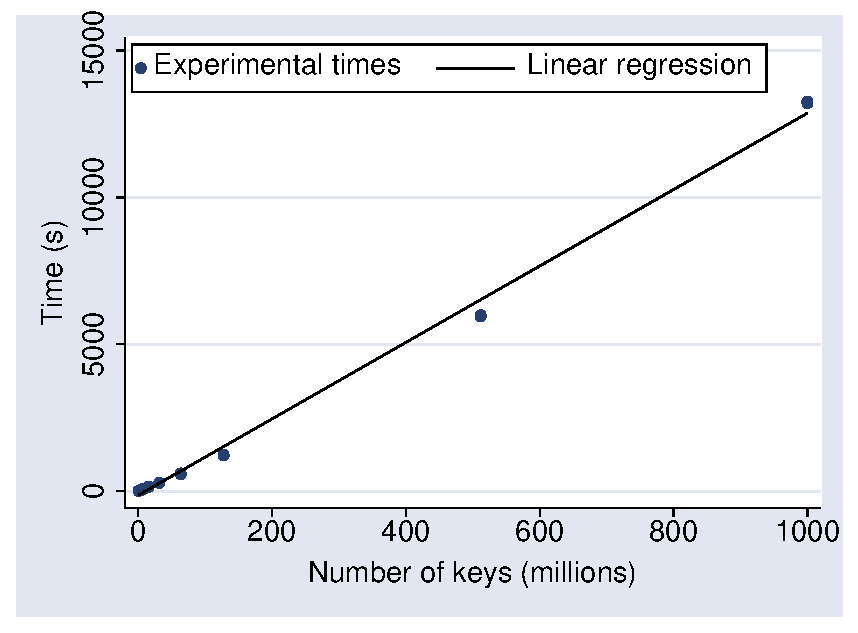
\includegraphics{figs/brz_temporegressao.eps}}}
%   \end{minipage}
%     \caption{Time versus number of keys in $S$. The solid line corresponds to 
% a linear regression model.}
% %obtained from the experimental measurements.}
%     \label{fig:temporegressao}
% \end{figure*}

Table~\ref{tab:medias} presents the runtime average for each $n$,
the respective standard deviations, and 
the respective confidence intervals given by 
the average time $\pm$ the distance from average time
considering a confidence level of $95\%$.
Observing the runtime averages one sees that 
the algorithm runs in expected linear time, 
as shown in~\cite{bkz05}. 

\vspace{-2mm}
\begin{table*}[htb]
\begin{center}
{\scriptsize
\begin{tabular}{|c|c|c|c|c|c|c|c|}
\hline
$n$ (millions)  & 1                 & 2                    & 4                  & 8                  & 16      & 32 \\
\hline
Average time (s)& $6.1 \pm 0.3$ & $12.2 \pm 0.6$   & $25.4 \pm 1.1$ & $51.4 \pm 2.0$ & $117.3 \pm 4.4$ & $262.2 \pm 8.7$\\
SD (s)          & $2.6$           & $5.4$              & $9.8$            & $17.6$           & $37.3$            & $76.3$  \\
\hline
\end{tabular}
\vspace{-1mm}
}
\end{center}
\caption{Internal memory based algorithm: average time in seconds for constructing a MPHF,
the standard deviation (SD), and the confidence intervals considering
a confidence level of $95\%$.}
\label{tab:medias}
\vspace{-4mm}
\end{table*}

% \enlargethispage{\baselineskip}
% \begin{table*}[htb]
% \begin{center}
% {\scriptsize
% (a)
% \begin{tabular}{|c|c|c|c|c|c|c|c|}
% \hline
% $n$ (millions)  & 1                 & 2                    & 4                  & 8                  & 16                 & 32 \\
% \hline
% Average time (s)& $6.119 \pm 0.300$ & $12.190 \pm 0.615$   & $25.359 \pm 1.109$ & $51.408 \pm 2.003$ & $117.343 \pm 4.364$ & $262.215 \pm 8.724$\\
% SD (s)          & $2.644$           & $5.414$              & $9.757$            & $17.627$           & $37.333$            & $76.271$  \\
% \hline
% \end{tabular}
% \\[5mm]  (b)
% \begin{tabular}{|l|c|c|c|c|c|}
% \hline
% $n$ (millions)   & 1                  & 2                  & 4                  & 8                   & 16             \\
% \hline % Part.      16 \%                 16 \%                 16 \%                18 \%                 20\%           
% Average time (s) & $6.927 \pm 0.309$  & $13.828 \pm 0.175$ & $31.936 \pm 0.663$ & $69.902 \pm 1.084$  & $140.617 \pm 2.502$  \\
% SD               & $0.431$            & $0.245$            & $0.926$            & $1.515$             & $3.498$         \\
% \hline
% \hline
% $n$ (millions)   & 32                  & 64                   & 128                    & 512                  & 1000            \\
% \hline % Part.      20 \%                 20\%                  20\%                      18\%                    18\%
% Average time (s) & $284.330 \pm 1.135$ & $587.880 \pm 3.945$  & $1223.581 \pm 4.864$   & $5966.402 \pm 9.465$ & $13229.540 \pm 12.670$  \\
% SD               & $1.587$             & $5.514$              & $6.800$                & $13.232$             & $18.577$            \\
% \hline
% \end{tabular}
% }
% \end{center}
% \caption{The runtime averages in seconds, 
% the standard deviation (SD), and
% the confidence intervals given by the average time $\pm$ 
% the distance from average time considering 
% a confidence level of $95\%$.}
% \label{tab:medias}
% \end{table*}

\enlargethispage{2\baselineskip}
Figure~\ref{fig:bmz_temporegressao} 
presents the runtime for each trial. In addition, 
the solid line corresponds to a linear regression model 
obtained from the experimental measurements.
As we can see, the runtime for a given $n$ has a considerable 
fluctuation. However, the fluctuation also grows linearly with $n$.

\begin{figure}[htb]
\vspace{-2mm}
\begin{center}
\scalebox{0.4}{\includegraphics{figs/bmz_temporegressao}}
\caption{Time versus number of keys in $S$ for the internal memory based algorithm.
The solid line corresponds to a linear regression model.}
\label{fig:bmz_temporegressao}
\end{center}
\vspace{-6mm}
\end{figure}

The observed fluctuation in the runtimes is as expected; recall that this
runtime has the form~$\alpha nZ$ with~$Z$ a geometric random variable with
mean~$1/p=e$.  Thus, the runtime has mean~$\alpha n/p=\alpha en$ and standard
deviation~$\alpha n\sqrt{(1-p)/p^2}=\alpha n\sqrt{e(e-1)}$. 
Therefore, the standard deviation also grows 
linearly with $n$, as experimentally verified 
in Table~\ref{tab:medias} and in Figure~\ref{fig:bmz_temporegressao}.

%\noindent-------------------------------------------------------------------------\\
%Comentario para Yoshi: Nao consegui reproduzir bem o que discutimos 
%no paragrafo acima, acho que vc conseguira justificar melhor :-). \\
%-------------------------------------------------------------------------\\

% Nivio: 29/jan/06
% Time-stamp: <Monday 30 Jan 2006 12:13:14pm EST yoshi@flare>
\subsection{Performance of the new algorithm}
\label{sec:performance}
%As we have done for the internal memory based algorithm, 

The runtime of our algorithm is also a random variable, but now it follows a
(highly concentrated) normal distribution, as we discuss at the end of this
section.  Again, we are interested in verifying the linearity claim made in
Section~\ref{sec:linearcomplexity}.  Therefore, we ran the algorithm for
several numbers $n$ of keys in $S$.

The values chosen for $n$ were $1, 2, 4, 8, 16, 32, 64, 128, 512$ and $1000$
million. 
%Just the small vector {\it size} must be kept in main memory,
%as we saw in Section~\ref{sec:memconstruction}.
We limited the main memory in 500 megabytes for the experiments.
The size $\mu$ of the a priori reserved internal memory area 
was set to 250 megabytes, the parameter $b$ was set to $175$ and
the building block algorithm parameter $c$ was again set to $1$.
In Section~\ref{sec:contr-disk-access} we show how $\mu$
affects the runtime of the algorithm. The other two parameters
have insignificant influence on the runtime.  

We again use a statistical method for determining a suitable sample size
%~\cite[Chapter 13]{j91}
to estimate the number of trials to be run for each value of $n$.  We got that
just one trial for each $n$ would be enough with a confidence level of $95\%$.
However, we made 10 trials.  This number of trials seems rather small, but, as
shown below, the behavior of our algorithm is very stable and its runtime is
almost deterministic (i.e., the standard deviation is very small).
 
Table~\ref{tab:mediasbrz} presents the runtime average for each $n$,
the respective standard deviations, and 
the respective confidence intervals given by 
the average time $\pm$ the distance from average time
considering a confidence level of $95\%$.
Observing the runtime averages we noticed that 
the algorithm runs in expected linear time, 
as shown in~Section~\ref{sec:linearcomplexity}.  Better still,
it is only approximately $60\%$  slower than our internal memory based algorithm.
To get that value we used the linear regression model obtained for the runtime of
the internal memory based algorithm to estimate how much time it would require
for constructing a MPHF for a set of 1 billion keys. 
We got 2.3 hours for the internal memory based algorithm  and we measured  
3.67 hours on average for our algorithm. 
Increasing the size of the internal memory area 
from 250 to 600 megabytes (see Section~\ref{sec:contr-disk-access}),
we have brought the time to 3.09 hours. In this case, our algorithm is 
just $34\%$  slower in this setup.

\enlargethispage{2\baselineskip}
\begin{table*}[htb]
\vspace{-1mm}
\begin{center}
{\scriptsize
\begin{tabular}{|l|c|c|c|c|c|}
\hline
$n$ (millions)   & 1                  & 2                  & 4                  & 8                   & 16             \\
\hline % Part.      16 \%                 16 \%                 16 \%                18 \%                 20\%           
Average time (s) & $6.9 \pm 0.3$  & $13.8 \pm 0.2$ & $31.9 \pm 0.7$ & $69.9 \pm 1.1$  & $140.6 \pm 2.5$  \\
SD               & $0.4$            & $0.2$            & $0.9$            & $1.5$             & $3.5$         \\
\hline
\hline
$n$ (millions)   & 32                  & 64                   & 128                    & 512                  & 1000            \\
\hline % Part.      20 \%                 20\%                  20\%                      18\%                    18\%
Average time (s) & $284.3 \pm 1.1$ & $587.9 \pm 3.9$  & $1223.6 \pm 4.9$   & $5966.4 \pm 9.5$ & $13229.5 \pm 12.7$  \\
SD               & $1.6$             & $5.5$              & $6.8$                & $13.2$             & $18.6$            \\
\hline

\end{tabular}
\vspace{-1mm}
}
\end{center}
\caption{Our algorithm: average time in seconds for constructing a MPHF,
the standard deviation (SD), and the confidence intervals considering 
a confidence level of $95\%$.
}
\label{tab:mediasbrz}
\vspace{-5mm}
\end{table*}

Figure~\ref{fig:brz_temporegressao}
presents the runtime for each trial. In addition, 
the solid line corresponds to a linear regression model 
obtained from the experimental measurements.
As we were expecting the runtime for a given $n$ has almost no 
variation.

\begin{figure}[htb]
\begin{center}
\scalebox{0.4}{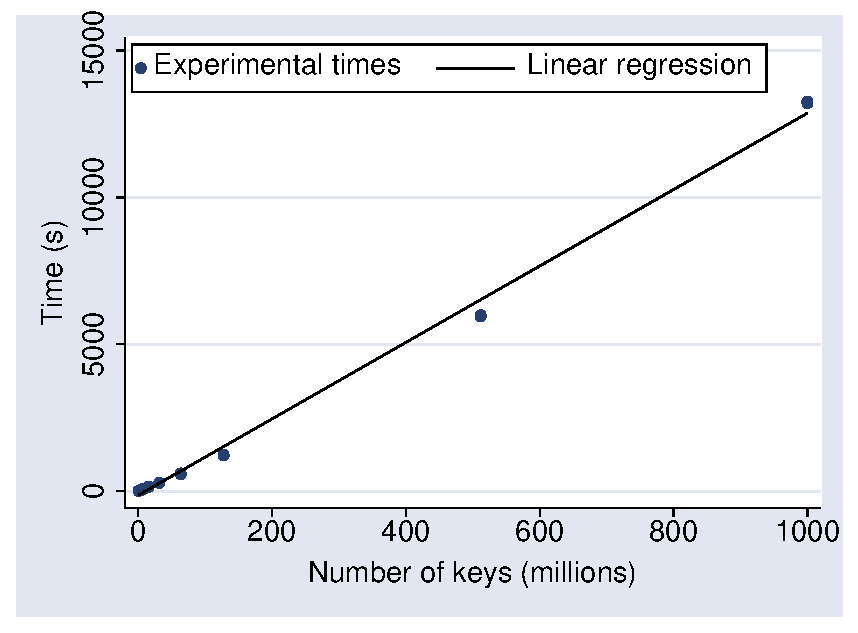
\includegraphics{figs/brz_temporegressao}}
\caption{Time versus number of keys in $S$ for our algorithm. The solid line corresponds to 
a linear regression model.}
\label{fig:brz_temporegressao}
\end{center}
\vspace{-9mm}
\end{figure}

An intriguing observation is that the runtime of the algorithm is almost
deterministic, in spite of the fact that it uses as building block an
algorithm with a considerable fluctuation in its runtime.  A given bucket~$i$,
$0 \leq i < \lceil n/b \rceil$, is a small set of keys (at most 256 keys) and,
as argued in Section~\ref{sec:intern-memory-algor}, the runtime of the
building block algorithm is a random variable~$X_i$ with high fluctuation.
However, the runtime~$Y$ of the searching step of our algorithm is given
by~$Y=\sum_{0\leq i<\lceil n/b\rceil}X_i$.  Under the hypothesis that
the~$X_i$ are independent and bounded, the {\it law of large numbers} (see,
e.g., \cite{j91}) implies that the random variable $Y/\lceil n/b\rceil$
converges to a constant as~$n\to\infty$.  This explains why the runtime of our
algorithm is almost deterministic.



% Nivio: 29/jan/06
% Time-stamp: <Sunday 29 Jan 2006 11:58:28pm EST yoshi@flare>
\vspace{-2mm}
\subsection{Controlling disk accesses}
\label{sec:contr-disk-access}

In order to bring down the number of seek operations on disk
we benefit from the fact that our algorithm leaves almost all main
memory available to be used as disk I/O buffer. 
In this section we evaluate how much the parameter $\mu$ 
affects the runtime of our algorithm.
For that we fixed $n$ in 1 billion of URLs,
set the main memory of the machine used for the experiments 
to 1 gigabyte and used $\mu$ equal to $100, 200, 300, 400, 500$ and $600$
megabytes. 

\enlargethispage{2\baselineskip}
Table~\ref{tab:diskaccess} presents the number of files $N$,
the buffer size used for all files, the number of seeks in the worst case considering
the pessimistic assumption mentioned in Section~\ref{sec:linearcomplexity}, and 
the time to generate a MPHF for 1 billion of keys as a function of the amount of internal 
memory available. Observing Table~\ref{tab:diskaccess} we noticed that the time spent in the construction
decreases as the value of $\mu$ increases. However, for $\mu > 400$, the variation 
on the time is not as significant as for $\mu \leq 400$. 
This can be explained by the fact that the kernel 2.6 I/O scheduler of Linux
has smart policies  
for avoiding seeks and diminishing the average seek time 
(see \texttt{http://www.linuxjournal.com/article/6931}).
\begin{table*}[ht]
\vspace{-2mm}
\begin{center}
{\scriptsize
\begin{tabular}{|l|c|c|c|c|c|c|}
\hline
$\mu$ (MB)                                                        & $100$                        & $200$                       & $300$                       & $400$                       & $500$                       & $600$ \\
\hline
$N$ (files)                                                       & $619$                        & $310$                       & $207$                       & $155$                       & $124$                       & $104$ \\
%\hline
\textbaht~(buffer size in KB)                                     & $165$                        & $661$                       & $1,484$                     & $2,643$                     & $4,129$                     & $5,908$ \\
%\hline
$\beta$/\textbaht~(\# of seeks in the worst case)                 & $384,478$                    & $95,974$                    & $42,749$                    & $24,003$                    & $15,365$                    & $10,738$ \\
% \hline
% \raisebox{-0.2em}{\# of seeks performed in}                       & \raisebox{-0.7em}{$383,056$} & \raisebox{-0.7em}{$95,919$} & \raisebox{-0.7em}{$42,700$} & \raisebox{-0.7em}{$23,980$} & \raisebox{-0.7em}{$15,347$} & \raisebox{-0.7em}{$xx,xxx$} \\
% \raisebox{0.2em}{statement 1.3 of Figure~\ref{fig:readingbucket}} &                              &                             &                             &                             &                             &       \\
% \hline
Time (hours)                                                      & $4.04$                       & $3.64$                      & $3.34$                      & $3.20$                      & $3.13$                      & $3.09$      \\
\hline
\end{tabular}
\vspace{-1mm}
}
\end{center}
\caption{Influence of the internal memory area size ($\mu$) in our algorithm runtime.}
\label{tab:diskaccess}
\vspace{-14mm}
\end{table*}



% \begin{table*}[ht]
% \begin{center}
% {\scriptsize
% \begin{tabular}{|l|c|c|c|c|c|c|c|c|c|c|c|}
% \hline
% $\mu$ (MB)                                                        & $100$                        & $150$                        & $200$                       & $250$                       & $300$                       & $350$                       & $400$                       & $450$                       & $500$                       & $550$                       & $600$ \\
% \hline
% $N$ (files)                                                       & $619$                        & $413$                        & $310$                       & $248$                       & $207$                       & $177$                       & $155$                       & $138$                       & $124$                       & $113$                       & $103$ \\
% \hline
% \textbaht~(buffer size in KB)                                     & $165$                        & $372$                        & $661$                       & $1,033$                     & $1,484$                     & $2,025$                     & $2,643$                     & $3,339$                     &                             &                             &       \\
% \hline
% \# of seeks (Worst case)                                          & $384,478$                     & $170,535$                    & $95,974$                    & $61,413$                    & $42,749$                    & $31,328$                    & $24,003$                    & $19,000$                    &                             &                             &       \\
% \hline
% \raisebox{-0.2em}{\# of seeks performed in}                       & \raisebox{-0.7em}{$383,056$} & \raisebox{-0.7em}{$170,385$} & \raisebox{-0.7em}{$95,919$} & \raisebox{-0.7em}{$61,388$} & \raisebox{-0.7em}{$42,700$} & \raisebox{-0.7em}{$31,296$} & \raisebox{-0.7em}{$23,980$} & \raisebox{-0.7em}{$18,978$} & \raisebox{-0.7em}{$xx,xxx$} & \raisebox{-0.7em}{$xx,xxx$} & \raisebox{-0.7em}{$xx,xxx$} \\
% \raisebox{0.2em}{statement 1.3 of Figure~\ref{fig:readingbucket}} &                              &                              &                             &                             &                             &                             &                             &                             &                             &                             &       \\
% \hline
% Time (horas)                                                      & $4.04$                          & $3.93$                       & $3.64$                      & $3.46$                      & $3.34$                      & $3.26$                      & $3.20$                      & $3.13$                      &                             &                             &       \\
% \hline
% \end{tabular}
% }
% \end{center}
% \caption{Influence of the internal memory area size ($\mu$) in our algorithm runtime.}
% \label{tab:diskaccess}
% \end{table*}



% \begin{table*}[htb]
% \begin{center}
% {\scriptsize
% \begin{tabular}{|l|c|c|c|c|c|}
% \hline
% $n$ (millions)   & 1                  & 2                  & 4                  & 8                   & 16             \\
% \hline % Part.      16 \%                 16 \%                 16 \%                18 \%                 20\%           
% Average time (s) & $14.124 \pm 0.128$ & $28.301 \pm 0.140$ & $56.807 \pm 0.312$ & $117.286 \pm 0.997$ & $241.086 \pm 0.936$  \\
% SD               & $0.179$            & $0.196$            & $0.437$            & $1.394$             & $1.308$         \\
% \hline
% \hline
% $n$ (millions)   & 32                  & 64                   & 128                    & 512                    & 1000            \\
% \hline % Part.      20 \%                 20\%                  20\%                      18\%                    18\%
% Average time (s) & $492.430 \pm 1.565$ & $1006.307 \pm 1.425$ & $2081.208 \pm 0.740$   & $9253.188 \pm 4.406$ & $19021.480 \pm 13.850$  \\
% SD               & $2.188$             & $1.992$              & $1.035$                & $ 6.160$             & $18.016$            \\
% \hline

% \end{tabular}
% }
% \end{center}
% \caption{The runtime averages in seconds, 
% the standard deviation (SD), and
% the confidence intervals given by the average time $\pm$ 
% the distance from average time considering 
% a confidence level of $95\%$.
% }
% \label{tab:mediasbrz}
% \end{table*}


\end{document}
